\chapter{Theory}\label{cha:litterature}

This chapter introduces three anomaly detection techniques that can be used for condition monitoring, and methods for feature extraction and dimensionality reduction to be used in addition to the anomaly detection techniques. 


\section{Anomaly detection}\label{sec:novelty_detection}
    \cite{Pimentel2014} defines anomaly detection as the task of classifying test data that in some way differs from data used for training, hence this is one obvious approach to condition monitoring. This is like a one-sided test or one class classification. This means that one is not training on data that represents fault, only on data sampled from normal operation. As a model describing the normal operation of the system is learned, it is essential that one has samples of normal system behavior for all the possible states of operation. Anomaly detection avoids the issue with finding data that represents all possible failure modes. Such techniques are very valuable for industrial applications, where the need for failure detection is great, but identifying all possible failure modes and collecting data to represent them can be difficult and very costly. It is much easier to get measurements from a machine during normal operation, than during failure, and it is in many cases close to impossible to obtain as many samples of negative or faulty behavior as of normal behavior. \cite{Tarassenko2009} claims that modern high-integrity systems are so complex that they introduce many possible failure modes that are not very well captured by the instrumentation available. This can be verified by visiting a hydroelectric power plant. There is much instrumentation, and many alarms for different components, but all of these are linked to well-known failure modes. Anomaly detection introduces the possibility to detect unknown abnormalities. It is, however, important to notice that anomaly detection methods are prone to suffer from a higher rate of false positives than when abnormal data is available for training \cite{Latecki}. The performance of the anomaly detection is dependent on the choice of parameters, and it is essential to keep in mind whether it is false negatives or false positives that are of the highest concern 
    
    Since anomaly detection techniques are based on "normal" system behavior, they should, in theory, be able to detect any failure mode that can occur, if provided with the correct process information. Adding process signals that are not known to be connected to any of the known failure modes can be beneficial for such methods. This also makes sense when one does not know what to look for. One wants all possible information available. This leads to a significant remark, only getting a notification that an anomaly is observed, does not provide very much information. For these techniques to have any real value, one needs to be able to trace which component the anomaly comes from, and the magnitude of the anomaly. Once the anomaly detection techniques are trained, new data are given a novelty score based on how well they compare to the normal description of the system. This score can then be compared to a threshold, and the data will be marked as normal or abnormal. Using anomaly detection techniques avoids having to create data that represent the failure modes as seen in \ref{sec:cm}. This means that the methods are more straightforward to generalize and adapt to new uses. 

    Many of the techniques in the following sections are based on the suggestions from \cite{Pimentel2014} which provides an extensive review of novelty detection. 

\section{Reducing the input space}\label{sec:reduce_features}
    As the size of the input grows, the complexity and runtime of the techniques grow with it. It can become necessary to reduce the input space of the anomaly detection techniques to ensure reasonable run time. Interpreting and visualizing data of high dimensions is difficult. The feature size also introduces issues regarding memory and algorithm runtime, \cite{Guyon2003} and \cite{Dy2004}. Reducing the complexity of the problem is heavily correlated with reducing the number of features. Feature selection techniques can also reveal unknown plant dynamics which can help to understand why some components fail.
    
    "The problem is that not all features are important. Some of the features may be redundant, some may be irrelevant, and some can even misguide clustering results" from \cite{Dy2004} sums up one of the issues with datasets with many features. A concrete example of this is shown in Figure \ref{fig:feature_selection}, her one can clearly see that $X_2$ does not provide any information on how the data points are clustered. Including this feature in a learning algorithm does not provide any information about the two classes found in the dataset, hence in the best case, the performance will be the same as if only $X_1$ was used. This is supported by \cite{Liu2010} that states that some features can be removed without lowering the performance of a learning algorithm.
    
    \begin{figure}
        \centering
        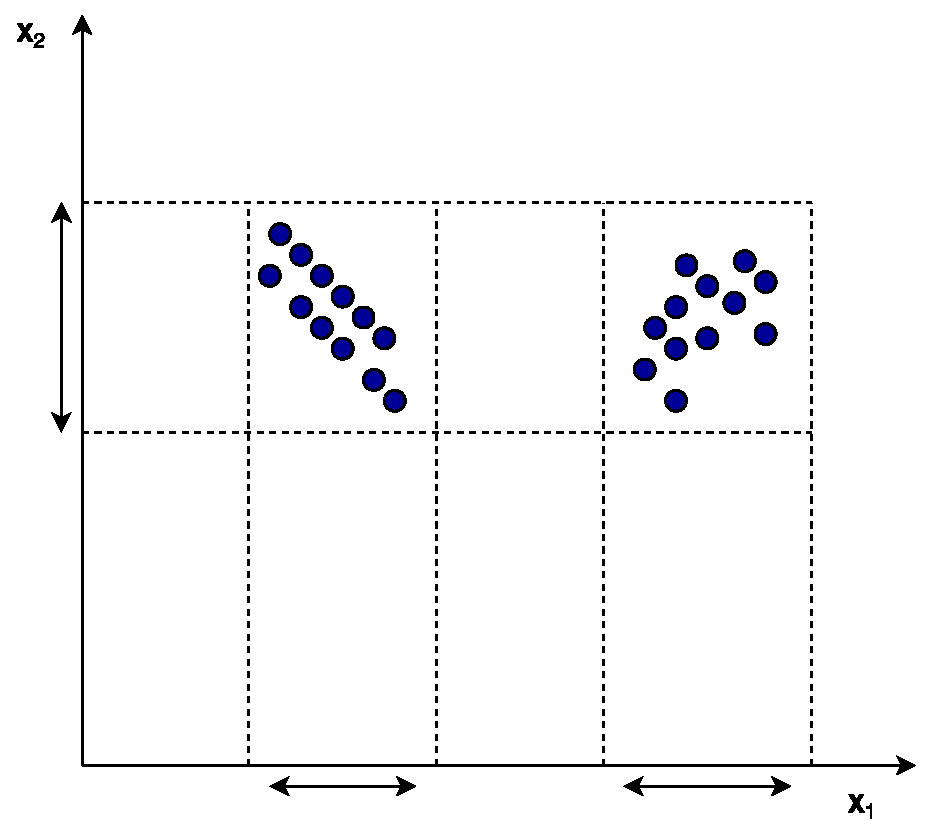
\includegraphics[width=0.5\textwidth]{report/figures/techniques/feature_selection.pdf}
        \caption{Example of a dataset with two features, one relevant and one irrelevant feature}
        \label{fig:feature_selection}
    \end{figure}
    
    There are two main techniques for reducing the input space, feature selection and dimensionality reduction. The former, try to remove the least informative and the redundant features from the feature set. The latter creates new features either as linear or non-linear combinations of the original feature set, hence one can remove the dimensions with little variance. Feature selection is again separated into a supervised and non-supervised selection. In the supervised case, one has a set of features and a target variable, hence one want to keep the features that are related to the target variable. For unsupervised feature selection, there is no target variable to help remove uninformative or redundant features, and other factors must be used for selection.
    
    
    \subsection{Filter, wrapper and embedded methods}\label{subsec:filter_wrapper_embedded}
        The different classes or types of methods for feature reduction are split into three groups, filter, wrapper and embedded methods. This section will give a short introduction to each of them.
        According to \cite{Liu2010} filter methods are methods that perform feature selection separate from the learning algorithm, and hence can be used no matter which learning algorithm is applied later. The wrapper methods, however, need a predetermined learning algorithm. The features are then selected based upon the performance of the chosen algorithm.  Finally, the embedded methods incorporate the selection of features in the training of the learning algorithms model. \cite{Liu2010} also states that since the filter methods are independent of the learning algorithm they are not biased with regard to the algorithm, this means that filter methods are to prefer when the learning algorithms are not known beforehand. 
\section{Supervised feature selection}\label{sec:sup_feat_select}
    Supervised feature selection can be used when one has a target to track. This means that one needs to identify a process signal or a function of a process signal of interest which one want to trace in the other process variables. An example is anomaly detection for a bearing. By using process variables from the bearing such as vibration and temperature, one can find other process variables that are in some way related to the targets. This section introduces two supervised feature selection methods. 
    % As seen in chapter \ref{cha:data} the control problems with the needles can be observed in the difference or the RMSE between the pairwise controlled needles. Using the RMSE between the needles as a target variable enables the use of supervised feature selection algorithms. 
    
    
    \subsection{K-best using correlation and  mutual information}\label{subsec:K-best_feat_select}
    
        Mutual information (MI), \cite{Kraskov2004} and \cite{Peng2005} explains how dependent or inversely how independent two variables are. It gives an understanding of how much knowing something about one variable reduces the uncertainty about the other. If two variables are completely independent, their corresponding MI. 
        
        The MI is defined as
        \begin{align}\label{eq:tech_MI}
                MI(X,Y) = \int \int p(x,y) \log \frac{p(x,y)}{p_x(x)p_y(y)},
        \end{align}
        where $x$ and $y$ are the two variables to compare, and $p_x(x)$ and $p_y(y)$ are their corresponding probability density functions. One benefit from MI is that does not only find linear correlation between two variables. In other words, it finds dependencies between variables not necessarily shown in correlation, meaning that this serves as complementary technique to using co-variance or correlation for feature selection, \cite{Li}. The K features with highest MI will be chosen. 
        
        
        The K-best features can also be selected using the above-mentioned correlation. The correlation between a feature and the target variable is found as  
        \begin{align}
            corr(X,Y) = \frac{cov(X,Y}{\sigma_x\sigma_y} = \frac{E[(X-\mu_x)(Y-\mu_y)]}{\sigma_x\sigma_y}.
        \end{align}
        Here the K features with highest correlation with the target variable will be chosen. 
        
\section{Unsupervised feature selection}\label{sec:unsup_feat_reduc}
    Unsupervised feature selection is harder than supervised feature selection. The lack of a target variable removes the ability to interpret which variable dynamics that are important easily. Still, the need to reduce the feature set is prominent. \cite{Dy2004} describes the problem as follows, "The goal of feature selection for unsupervised learning is to find the smallest feature subset that best uncovers “interesting natural” groupings (clusters) from data according to the chosen criterion." The chosen criterion defines what is thought to be interesting natural groupings. There is no golden rule for defining this criterion, and a subset that is good for one purpose might not be relevant for others. Two possible methods for unsupervised feature selection follows.
    
    
    \subsection{K-best using variance threshold}\label{subsec:var_thres}
        Variance threshold removes merely the features with the lowest variance. According to \cite{He2005} it is one of the most straightforward evaluation methods for unsupervised selection. One of the drawbacks of using variance to select features is that there might be many features with large variances that is non-informative with what one is looking for. The algorithm is very simple, and it returns the k features that have the highest variance. 
        
    
    \subsection{Laplacian score}\label{subsec:lapl_score}
        Laplacian score for feature selection was proposed as an alternative to unsupervised feature selection by \cite{He2005}. The method builds upon the assumption that features belonging to the same class or grouping can be found close together. The features are evaluated based on how well locality is preserved, which is found by the Laplacian score. The Laplacian score is calculated for each feature. A short introduction to the method is described below. More details is found in \cite{He2005}. 
        
        Laplacian score is based on Laplacian Eigenmaps, which is an algorithm for dimensionality reduction. The algorithm creates a nearest neighbors graph with a node for each sample of each feature. Hence the dimension becomes $m$ times the number of features. Two nodes share an edge if they are among the k-nearest neighbors to each other, meaning that k is one of the tunable parameters for this algorithm. Each edge is then given a weight based on the Gaussian radial basis function;
        
        \begin{align}\label{eq:tech_LS}
            W_{i,j} = e^-{\frac{||{\bm{X_i}-\bm{X_j}}^2||}{t}},
        \end{align}
        
where t is another tunable parameter. Then a graph Laplacian is computed which then again is used to calculate a Laplacian score. As mentioned the algorithm has two tunable parameters. The main reason for choosing Laplacian score as one of the unsupervised feature selection methods is that it can compare and rate features against each other. This introduces a new dimension compared to the more naive variance threshold algorithm that only looks at one feature at a time. 
    

\section{Dimensionality reduction}\label{sec:dim_red}
    One of the issues with feature reduction is that the features that are removed may hold information that could help the learning algorithm. In dimensional reduction, the feature set is used to create new features which means that a new reduced feature space of dimension n can hold the same amount of information as the original feature space of size m, $m>n$.

    \subsection{Principal component analysis}\label{subsec:PCA}
        Principal component analysis (PCA) is a popular technique used for dimensional reduction. PCA is an orthogonal transformation that takes a set of possibly correlated variables, and transforms them into a set of noncorrelated components, effectively reducing the dimensions of the data. These new dimensions are known as principal components. There are several different algorithms that can be used to calculate the principal components, one of them is singular value decomposition or SVD. SVD decomposed the data into eigenvalues and eigenvectors. The larger an eigenvalue is, the better its corresponding eigenvector capture the variance of the data. All eigenvectors are orthogonal, this means that each vector introduces an entirely new dimension. In a high dimensional dataset with many features, there will most likely be features that are fairly similar. Figure \ref{fig:tech:PCA} shows intuitively how the PCA algorithm works. Data samples from a dataset with three features are shown in the plot. As the principal components in red and green shows, most of the variance in the samples can be represented using only one dimension. Adding the second dimension, only small residuals might be left. This illustrates how the PCA algorithm operates. 
        
        \begin{figure}
            \centering
            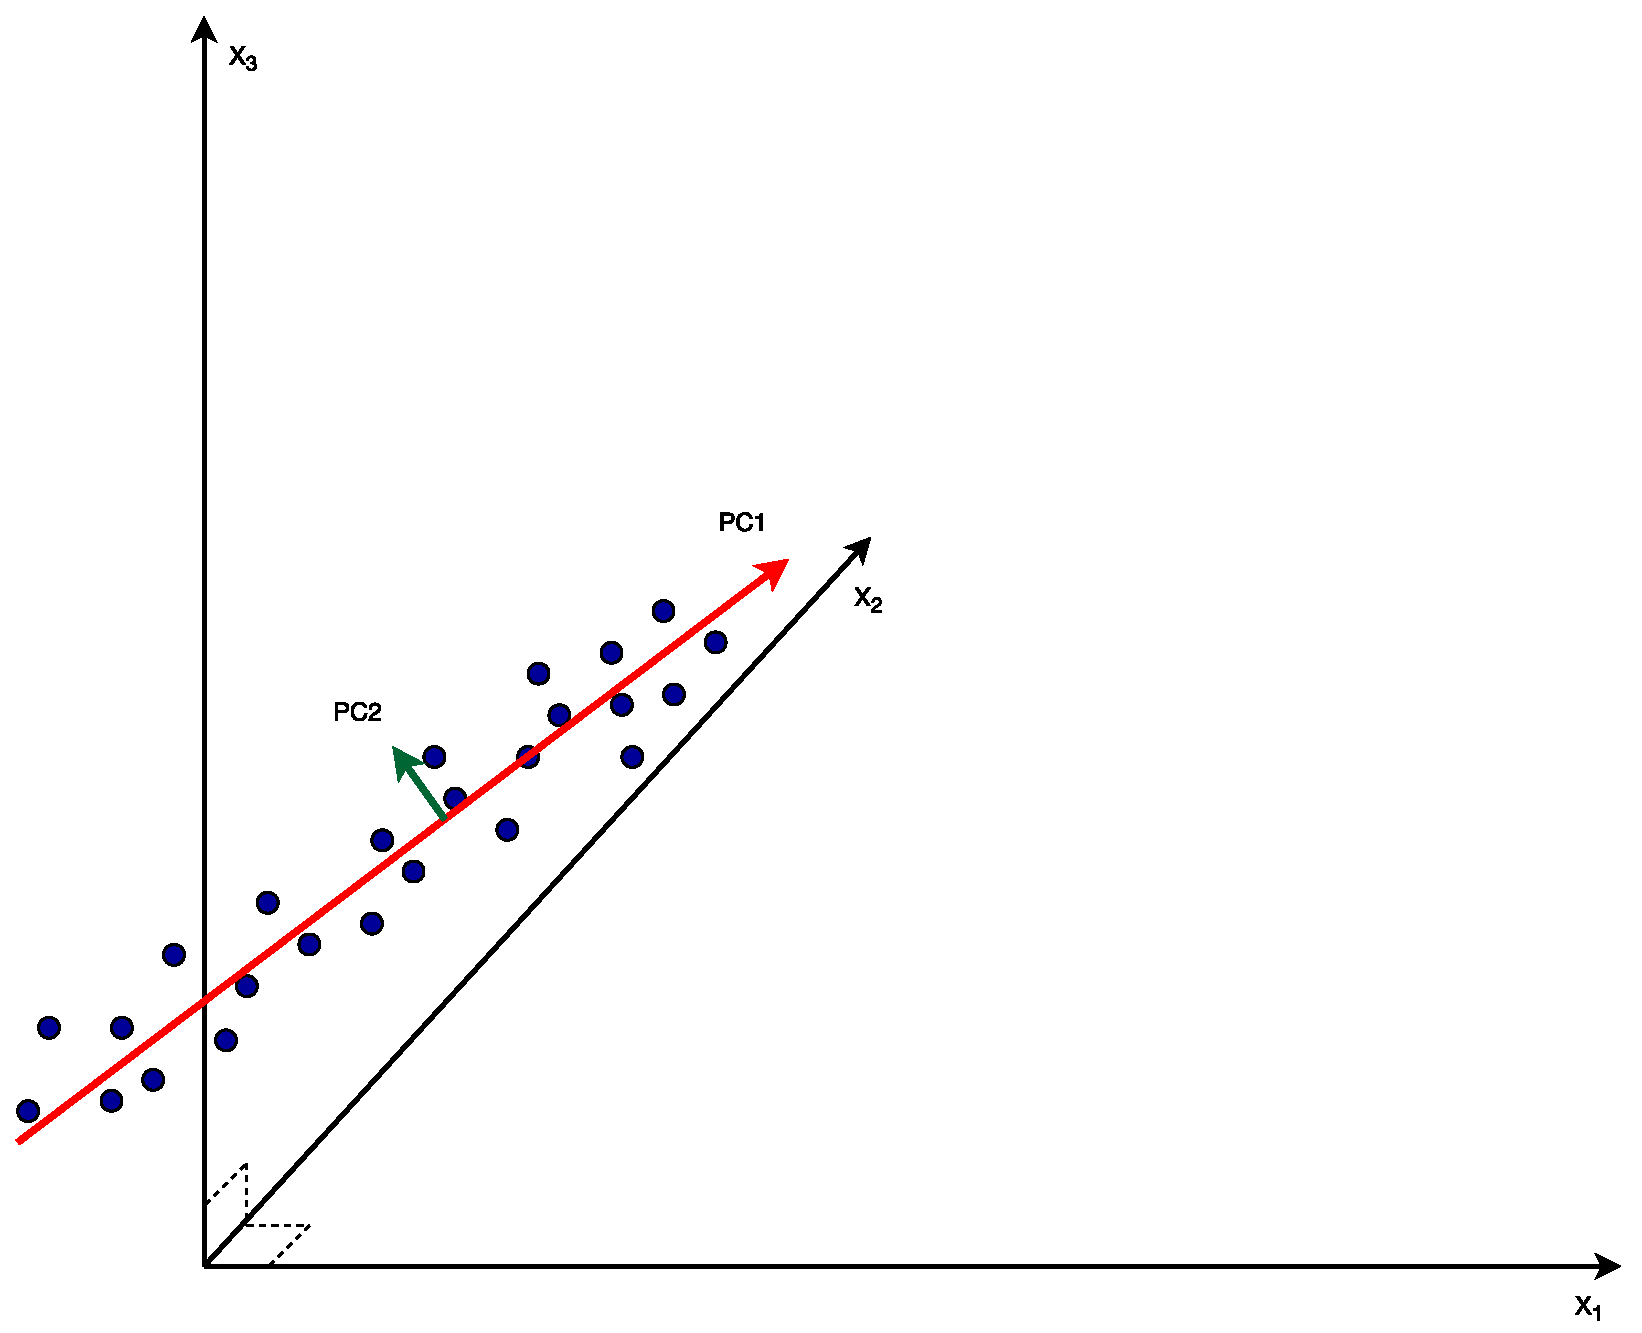
\includegraphics[width=\textwidth]{report/figures/techniques/PCA.pdf}
            \caption{Illustration of principal component analysis. The two principal components are seen in red and green. Using only PC1 most of the variance in the data is still kept.}
            \label{fig:tech:PCA}
        \end{figure}
        
        

    
    \subsection{Kernel principal component analysis}\label{subsec:kernelPCA}
        Kernel PCA builds upon the PCA algorithm explained above, but it introduces a new trick. Where PCA is only able to create new features from linear combinations of the original feature set, kernel PCA uses the kernel trick to enable non-linear combinations as well. Take a two-dimensional dataset containing samples from two different classes.  These classes are only linearly separable if the classes can be separated by a line. If one class surrounds the other class, there is no way to linearly separate the two classes in two dimensions. However, by extending the sample space into three dimensions, it might now be possible to separate the two classes with a hyperplane. Hence making a non-linear separation of the two classes possible, by still using linear methods. If the datasets are large, transforming all samples into a higher dimension can become computationally heavy. The kernel trick solves this problem without having to transform the samples. The kernel PCA extends the original PCA to a higher dimension using the kernel trick, enabling the extraction of nonlinear components.  
    
        By mapping the original data nonlinearly into a new feature space $F$ $\phi(\bm{x_1})$, and by performing PCA in this new feature space, one can get nonlinear principal components.


\section{Anomaly detection techniques}
    In this section, three different techniques for anomaly detection is presented. SVM is a classifying algorithm that automatically classifies data as either normal or an anomaly. \cite{Selak2014} uses SVM for condition monitoring. One Class Support Vector Machine (OCSVM) is presented as it only needs normal training data, removing the need for artificially creating data for known failure modes. Kernel density estimation (KDE) is a method for estimating the probability density function or pdf of a set of variables. New data can then be evaluated on how well it fits the learned pdf. Long short term memory recurrent neural network is neural network designed for learning time series data. 

    \subsection{One class support vector machine}\label{subsec:OCSVM}
    
            The following section is a based on \cite{Aasnes2017} and \cite{Hastie}. 
            
            SVMs can be used for data belonging to one or more classes. The SVM algorithm defines a hyperplane that best separates two different classes. Hence data is labeled normal or abnormal based on which side of the hyperplane it lays. In anomaly detection only normal data is available. Hence one has no negative data to help to fit the hyperplane. SVM is capable of separating data both linearly and non-linearly. A kernel function, or a similarity function, describes how similar two feature vectors are by taking the inner product of the two samples in a higher dimensional space. The kernel function does this without having to transform the data into this dimension explicitly. Two commonly used kernels are the Gaussian kernel
            \begin{align}
                K_g(\bm x^{1},\bm x^{2}) = e^{\frac{\norm{\bm x^{1}-\bm x^{2}}^2}{2\sigma^2}}, 
                \label{svm:gauss}
            \end{align}
            and the polynomial kernel
            \begin{align}
                K_p(\bm x^{1},\bm x^{2}) = (\bm x^{1T}\bm x^{2} + \alpha)^\beta.
                \label{svm:poly}
            \end{align}
           These are just two of many examples. The Gaussian or RBF kernell is a good first choice if you know that you have a nonlinear boundary, but don't know exactly what shape the boundary will take.
    
            \begin{align}
                f(\bm x) = \beta_0 + \bm \beta^T\bm x = 0,
                \label{svm:hyper}
            \end{align}
            defines a hyperplane. For any two feature vectors $\bm x^{[1]},\bm x^{[2]}$ that lie in or on the hyperplane where $\bm \hat x = \bm x^{[1]} - \bm x^{[2]}$, gives  $\bm \beta^T \bm \hat x = 0 $ and hence, $\bm \beta$ is a scalar multiplication of the normal vector to the hyperplane. Where
            \begin{align}
                \bm \beta^* = \frac{\bm \beta}{\norm{\bm \beta}}
                \label{svm:norm}
            \end{align}
            is the normal vector. Inserting any feature point $\bm x_0$ that lies on or in the hyperplane defined by Equation \ref{svm:hyper}, yields $\bm \beta^T\bm x_0 = -\bm \beta_0$. By using $\bm x_0$ as any feature vector from origo to the hyperplane and the normal vector $\bm \beta^*$, the distance for any given feature vector $\bm x$ to the hyperplane is given by
            \begin{align}
                \bm \beta^{*T}(\bm x - \bm x_0) = & \frac{\bm \beta^T}{\norm{\bm \beta}} (\bm x - \bm x_0) \nonumber \\
                % = & \frac{1}{\norm{\bm \beta}}(\bm \beta^T\bm x- \bm \beta^T\bm x_0) \nonumber \\
                % = & \frac{1}{\norm{\bm \beta}}(\bm \beta^T\bm x + \bm \beta_0) \nonumber \\
                = & \frac{1}{\norm{f'(\bm x)}}f(\bm x).
                \label{svm:dist}
            \end{align}
            
            A decision rule 
            \begin{align}
                y^i(\bm x^{iT} \bm \beta + \beta_0) \geq 0 
                \label{svm:decision}
            \end{align}
            can then be created using the hyperplane. Since there are two classes they are defined as $y_0 = 1$ and $y_1 = -1$. The decision rule tells which class a feature vector belongs to. Note that points belonging to the negative class should yield negative distance to the hyperplane, and hence the decision rule ensures that all points are classified correctly.
            
            Now that an expression for the distance from a hyperplane to any given feature vector in the feature space is defined, one can look at how to find the optimal hyperplane to separate the two classes. The margin or the width between the two closest point from both classes can be defined as $M = \frac{2}{\norm{\bm \beta}}$, and hence maximizing the distance can be formulated as minimizing
            \begin{align}
                J(\bm \beta) = & \frac{1}{2}\norm{\bm \beta}^2 \nonumber \\
                 s.t \quad y^i(\bm \beta^T\bm x^i + \beta_0) \geq & 1 \quad \forall \enspace i.
                \label{svm:cost}
            \end{align}
            The constraint here ensures that every point is classified correctly. Having to classify all samples correctly can lead to a very complex boundary or hyperplane, in addition there is always a risk that data is labeled incorrectly. Therefore slack variables are added to enable some wrong classifications as seen in the updated minimization problem
            \begin{align}
                J(\bm \beta) = & \frac{1}{2}\norm{\bm \beta}^2  + C \sum_{i=1}^N \xi_i \nonumber \\
                 s.t \quad \xi_i \geq 0, y^i(\bm \beta^T\bm x^i + \beta_0) \geq & 1 - \xi_i \quad \forall \enspace i.
                \label{svm:cost}
            \end{align}
            % The solutution to the original SVM algorithm is found by a Lagrangian optimization problem which maximize distance between two classes as, 
            %  \begin{align}
            %     L = \sum_{i=1}^n  \alpha_i - \frac{1}{2} \sum_{i=1}^n \sum_{j=1}^n \alpha_i \alpha_j y^i y^j \bm x^{i}^T \bm x^j,
            %     \label{svm:dual}
            % \end{align}
            % or by 
            % \begin{align}
            %     L = \sum_{i=1}^n  \alpha_i - \frac{1}{2} \sum_{i=1}^n \sum_{j=1}^n \alpha_i \alpha_j y^i y^j K(\bm x^{i}, \bm x^j)
            % \end{align}
            % if the kernel trick is used. Here $\alpha$ are the parameters that defines the separating hyperplane, and it is constrained by having to correctly classify data to its original class. Both are a convex optimization problem which has the nice attribute of having a global maxima. This means that you will always find the best solution for the given parameters.
            
            In the case of OCSVM, \cite{Scholkopf2001}, there is only one class available, so the problem is formulated slightly different,
            \begin{align}
                \min \quad J(\bm \beta) = & \frac{1}{2}\norm{\bm \beta}^2  + \frac{1}{\nu N}\sum_{i=1}^N \xi_i - \rho \nonumber \\
                s.t \quad (\beta \cdot \phi(x_i) \geq & \rho - \xi_i \quad \forall \enspace i \nonumber \\
                \xi_i \geq & 0 \quad \forall \enspace i.
                \label{svm:cost_oc}
            \end{align}
            The main difference is the parameter $\nu$ wich serves as a upper fractional bound for accepted number of outliers, and as a lower bound for the fraction of support vectors used by the algorithm. $\rho$ is simply an offset. OCSVM is typically trained on normal data, fitting the decision boundary close to the normal data pattern. Anomalies that deviate from the normal data will then be found on the other side of the separating hyperplane, and classified as an anomaly.    
            % If your classes are not linearly separable in the feature space, maximization of Equation \ref{svm:dual} has no global solution. However as can be seen in Equation \ref{svm:dual} one want to minimize $\bm x_i^T  \bm x_j$. This term can then be replaced by one of the kernel functions defined above, which now enables separation in a higher dimensional space.
            
            % The final thing to remark is that not all datasets are entirely separable, to deal with this a slack variable is introduced into the optimization to allow miss-classification of some of the feature vectors. 
        
    
        % One issue with one class SVM combined with non labeled data is that hyperparameterization becomes hard. There is no out of the box scoring function that tells how well the classifier is performing. As long as one is working in two or three dimensions, it is possible to plot the decision boundary, and select parameterization based on visual observations. In higher dimensions, this becomes a problem. Therefore a new method is proposed used to reduce the number of hyperparameterizations to consider. A score is given to each of the parameterizations from
        
        % \begin{align}
        %     score = \abs\sigma + \mu + 100\frac{outliers}{inliers},
        % \end{align}
        % where the lower the score, the better the performance. $\sigma$ here represents the standard deviation of the distances from the decision boundary, $\mu$ is the unsigned distance to the decision boundary. These values were picked because the training data is said to be normal operation, and should not contain any outliers. However, this leads to the risk of a too general boundary where the classifier is no longer able to predict outliers. This means that the closer the boundary is to the samples in the training data, the higher the score. The final fraction of outliers and inliers is added to make sure that most of the data is classified as inliers. If not on runs the risk of fitting a very complex boundary which yields good distance measures for all samples, this will, however, lead to a large fraction of outliers which is not the case for the normal training data. 
        
        
    
    \subsection{Kernel density estimation}\label{subsec:kde}
        KDE, \cite{Latecki}, creates an estimate of the probability density function or pdf of the data. The data is then evaluated by how likely it is to belong to the estimated density function. This is a non-parametric technique meaning that the data is not assumed to take the shape of a given distribution. The probability density function is estimated using a set of kernels that are distributed across the data. The probability density is then estimated at each kernel location based on data that lie within a local neighborhood of the kernel. The density found at a point x within its neighboring n points is given by, 
        \begin{align}
            \hat{f}(x) = \frac{1}{n} \sum_{i=1}^n K_h(x-x_i)  = \frac{1}{nh} \sum_{i=1}^n K(\frac{x-x_i}{h}).
        \end{align}
        Here the $K()$ is the kernel function, and $h$ is a tunable hyperparameter for variance known as the bandwidth. This parameter smooths the distribution, the larger the bandwidth the smoother the density estimation becomes. Hence a too small bandwidth will lead to overfitting, and a too large bandwidth will lead to underfitting.   
        
        The kernel function can take on many forms, where the Gaussian kernel,
        \begin{align}
            K(x-x_i;h) = e^-\frac{||x-x_i||^2}{2h^2}
        \end{align}
        is the most commonly used. KDE is mentioned as a method for anomaly detection in \cite{Pimentel2014}. The distribution of normal data is modeled by KDE, and new data is evaluated on how likely it is to belong to the learned distribution.
        

    \subsection{Neural networks}
        The introduction to NN is based on \cite{Aasnes2017} and \cite{Hastie}. 
        \begin{figure}[h]
            \centering
            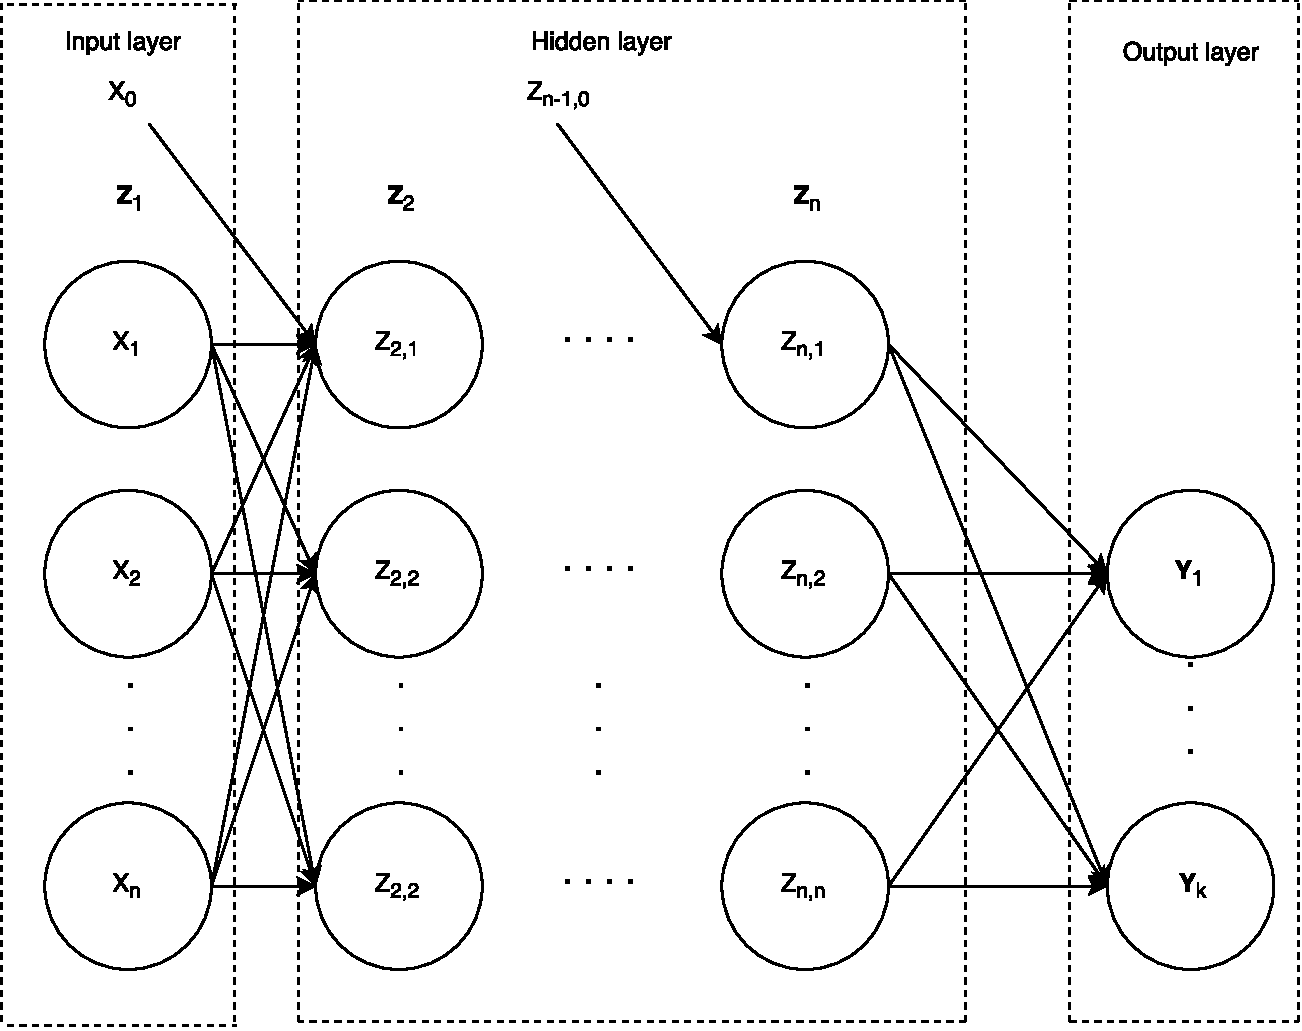
\includegraphics[width=0.8\textwidth]{report/figures/techniques/neural_network.pdf}
            \caption{A graph visualizing a N-level deep neural network. All hidden layers are fully connected. The size of the input and output layer depends on input size, and if the NN is used for regression or classification.}
            \label{fig:nn_fullnetwork}
        \end{figure}
        
        An NN is an n-class classification or regression algorithm. For anomaly detection, an NN can be trained to recreate the input of normal data. If the network is trained with enough normal data, it should be able to learn a good representation of patterns in this data. Abnormal data will in some way deviate from normal data, and hence its patterns are not familiar to the network. This will then result in recreated data that deviate more than normal from the input. This is also known as autoencoding. There are many types of NN specialized in solving specific tasks. Recurrent neural networks (RNN) are designed to learn trends seen over a period and are therefore a good option when working with time series. Within the recurrent NN, there is a type known as LSTM or long short-term memory, which has shown to outperform the standard RNN when it comes to long-horizon trends, \cite{Courville2016}. The following section introduces LSTM RNN by first introducing NN and RNN.  
        
        A visual representation of an NN is a graph with nodes and vertices as shown in Figure \ref{fig:nn_fullnetwork}. As seen, an NN consists of three parts, an input layer, a hidden layer, and an output layer. The input layer is the feature vectors for the data samples, the hidden layer does all the computation, and the output layer makes the prediction. An NN with only one layer and a limited number of neurons can approximate any function, \cite{Hastie}. This shows the ability an NN has for finding complex non-linear patterns.
        
        
        \begin{figure}[h]
            \centering
            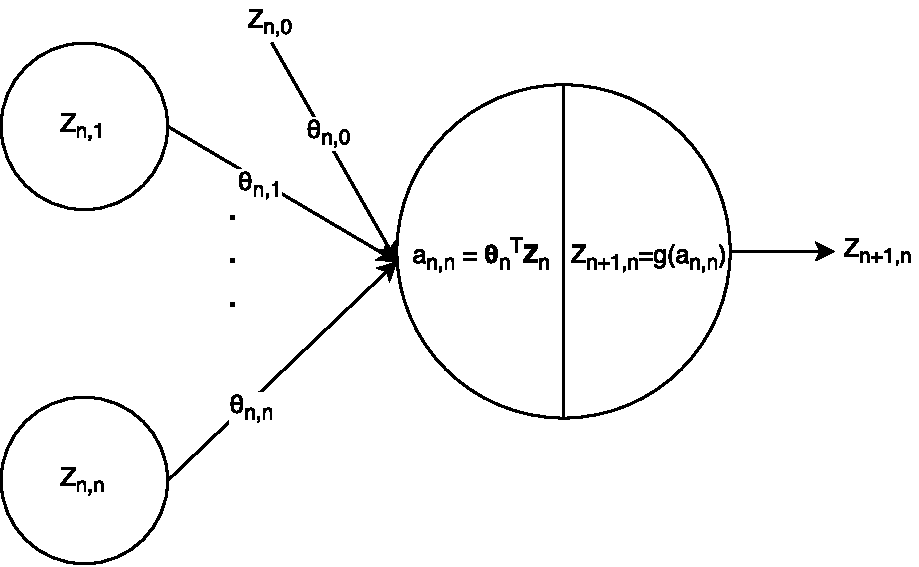
\includegraphics[width=0.5\textwidth]{report/figures/techniques/single_neuron.pdf}
            \caption{Visualization of a single neuron. The input is the output from the previous layer. The output is a scalar decided by the activation function $g(a)$}
            \label{fig:nn_neuron}
        \end{figure}
        
        Each of the nodes marked  $z_{n,n}$ seen in Figure \ref{fig:nn_fullnetwork} is known as a neuron. A single neuron is visualized in Figure \ref{fig:nn_neuron}. Each neuron does two things. First, it takes the dot product of the input vector and the weight vector, 
        
        \begin{equation}
            a = \bm \theta_n^T \bm Z_n,
            \label{eq:neuron_a}
        \end{equation}
        also shown in Figure \ref{fig:nn_neuron}. Then the output $Z_{n+1,n}$ is calculated 
        \begin{equation}
            Z_{n+1,n} = g(a_{n,n}).
            \label{eq:nn_activation}
        \end{equation}
        Here $g(a)$ is known as an activation function. There are many different options for activation functions, the most common are shown in Table \ref{tab:acitvations}. It is by using nonlinear activation functions, that a NN is enabled to approximate any function. If only linear functions are used, it can be verified that adding more layers does not but complicating a linear interpretation, \cite{Hastie}. The algorithm learns by updating the weights $\theta$ in each neuron.  
        
        
        %%%%%%%%% activation fucntions 
        % \begin{align}
        %     g_k(a) = a \textit{ identity function} \\
        %     g_k(a) = \frac{1}{1+e^{-a}} \textit{ sigmoid function} \\
        %     g_{k}(a) = \frac{e^{Tk}}{\sum_{i=1}^Ke^{Ti}} \textit{ softmax function} \\
        %     g_{k}(a) = \frac{e^a-e^{-a}}{e^a+e^{-a}} \textit{ tanh function} \\
        %     g_{k}(a) = max(a,0) \textit{ relu function}
        %     \label{eg:activations}
        % \end{align}
        
    \begin{table}[h]
        \centering
        \begin{tabular}{l l}
            \toprule
            \textbf{Function} & \\ \midrule
            Identity & $g_k(a) =a$ \\ 
            Sigmoid & $g_k(a) =\frac{1}{1+e^{-a}}$ \\ 
            Softmax & $g_k(a) =\frac{e^{Tk}}{\sum_{i=1}^Ke^{Ti}}$ \\ 
            Tanh & $g_k(a) =\frac{e^a-e^{-a}}{e^a+e^{-a}}$ \\ 
            Relu & $g_k(a) =max(a,0)$ \\ \bottomrule
        \end{tabular}
        \caption{Different activation functions}
        \label{tab:acitvations}
    \end{table}
        % \begin{align}
        %     z_{m} =  \sigma(\theta_{0m} + \bm \theta_m^T \bm z_{m-1}), \textit{m = 1,..,M} \nonumber \\
        %     \bm \hat y = g(\bm z_m) \nonumber \\
        %     \label{eq:fwdprop} 
        %     % \textit{where $\sigma()$ and g() are different activation function}\nonumber 
        % \end{align}
        % In the first layer, $\bm z_1 = \bm x$. For all the other layers each $z_m$ is given by the activations function of a bias term pluss the dot product of the inputs $\bm z$ and the weight $\bm \theta$. This means that for each layer there exists $m$ $\bm \theta$ vectors, which can be written as $\bm \Theta_m$. For the regression classifiers one only had one vector $\bm \theta$, but for a NN you end up with $m$ $\bm \Theta$ matrices. This gives a good indication on why a NN can approximate any given function. 
        The final layer calculates the output $\hat y$. The number of elements in the final layer depends as mentioned if it is classification or regression. For regression, the final layer usually only has one element, but for classification, it holds as many elements as there are classes. For binary classification, the Sigmoid function is typically used. For k-class classification, the Softmax function is used, and for regression the identity function.
        
        The weights of an NN are updated through forward and backward propagation. Forward propagation the input is fed through the mathematical operations in the network as seen in Figure \ref{fig:nn_neuron} and \ref{fig:nn_fullnetwork} and a set of labels or values are predicted. The cost function 
        \begin{align}
            E(\bm\Theta) = &\sum_{i=1}^M\frac{1}{2}(\hat{y} - y)^2 \nonumber,
            \label{nn:cost}
        \end{align}
        expresses how well the NN is able to correctly predict its output. The NN weights or coefficients $\bm \Theta = [\bm \Theta_1 ... \bm \Theta_n]$ are then updated through a step called backpropagation. The cost function is minimized as a function of the weigths. Gradient descent or another optimization algorithm is used to calculate each of the different parameters in $\bm \Theta$'s contribution to the cost. $\bm \Theta$ is updated as 
        \begin{align}
            \bm \Theta := & \bm \Theta - \alpha \nabla E(\bm \Theta) \nonumber \\
            \Theta_{ij} = & \Theta_{ij} - \alpha \sum_{k=1}^M \frac{\partial E_k}{\partial \Theta_{ij}} 
            \label{bp:1}
        \end{align}
        Here $\alpha$ is the learning rate, a value between [0,1]. The prediction errors are back-propagated to calculate the error in each neurons prediction. This prediction error is then used to update the corresponding weights for the neuron in the matrix $\bm \Theta$. A full mathematical proof can be found in \cite{Aasnes2017}
        
        % % Equation \ref{bp:1} to \ref{bp:9} shows how the partial derivative of the cost function is computed.   
        
        % \begin{align}
        %     \frac{\partial E}{\partial \Theta_{ji}} = \frac{\partial E}{\partial a_{ji}} \frac{\partial a_{ji}}{\partial \Theta_{ji}} \label{bp:2}.
        % \end{align}
        % Solving for the first term,
        % \begin{align}
        %     \delta_{ji} \coloneqq \frac{\partial E}{\partial a_{j,i}} = \sum_{k=1}^N \frac{\partial E}{\partial a_{j+1,k}} \frac{\partial a_{j+1,k}}{\partial a_{ji}} \label{bp:3}
        % \end{align}
        % where
        % \begin{align}
        %      \frac{\partial E}{\partial a_{j+1,k}} = \delta_{j+1,k}
        % \end{align}
        % and
        % \begin{align}
        %     \frac{\partial a_{j+1,k}}{\partial a_{ji}} = \frac{\partial \bm \theta_{j+1}^T \bm Z_{j+1}}{\partial a_{ji}}. \label{bp:4}
        % \end{align}
        % $\bm \theta_{j+1}^T \bm Z_{j+1}$ can be written as, 
        % \begin{align*}
        %     \bm \theta_{j+1}^T \bm Z_{j+1} = \Theta_{j+1,0}Z_{j+1,0} +\textit{ }..+ \textit{ }\Theta_{j+1,N}Z_{j+1,N} \nonumber \\
        %     = \Theta_{j+1,0}g(a_{j,0}) + \textit{ }.. +\textit{ }\Theta_{j+1,N}g(a_{j,N}). \label{bp:5}
        % \end{align*}
        % This gives, 
        % \begin{align}
        %     \frac{\partial a_{j+1,k}}{\partial a_{ji}} = \Theta_{j+1,i}\frac{\partial g(a_{j,i})}{\partial a_{ji}} =  \Theta_{j+1,i}g'(a_{ji}), \label{bp:6} 
        % \end{align}
        % which finally yields
        % \begin{align}
        %     \delta_{ji} = g'(a_{ji})\sum_{k=1}^N\delta_{j+1,k}\Theta_{j,k}. \label{bp:7}
        % \end{align}                    
        % Solving for the second term
        % \begin{align}
        %     a_{ji} = \bm \theta^T_i \bm Z_{i} \label{bp:10}
        % \end{align}
        % \begin{align}
        %     \frac{\partial a_{ji}}{\partial \Theta_{ij}} =  Z_{ji} \label{bp:8}
        % \end{align}
        % Gives the following equation
        % \begin{align}
        %     \frac{\partial E}{\partial \Theta_{ji}} = \delta_{ji}Z_{ji} \label{bp:9}
        % \end{align}
        
        The forward and backward-propagation steps are then iterated over until a given number of iterations are reached. A complete pass forward and backward of all training examples are known as one epoch. When the training set is large, it is often split into smaller batches to speed up calculations. The batch size explains how many samples are included in each forward and backward pass. Splitting the data into batches enables the algorithm to take advantage of parallelism, running the separate batches on separate CPUs or GPU's. How many epochs it takes for an NN to learn a good representation of the data can vary a lot. A technique called early stopping is introduced to ensure that the NN is stopped when the network no longer is showing sign of increased test predictions. Running an NN for too many epochs on a training set can cause the NN to overfit to the training data, giving poorer general performance than if stopped earlier.  
        
        
        A deep NN can learn more complex patterns than a shallow. However, the deeper the NN is, the more processing each iteration through it will take. Deep networks also increases the risk of overfitting. A good approach is to start with a shallow network, and increase the depth and width until you see that adding new layers, does not yield better performance. Other means to handle overfitting is regularization (making it costly to have large weights) and dropout. Dropout removes some edges between the neurons between each iteration, simplifying the network structure. 
        % To avoid overfitting the regularization term 
        % \begin{align}
        %     \frac{\lambda}{2} \sum_{km} \Theta_{km}^2  \nonumber \\
        %     = \frac{\lambda}{2}\bm \Theta^T \bm \Theta,
        %     \label{nn:overfit}
        % \end{align} 
        % is added to the cost function. The extra term in the cost function will penalize parameters $\neq 0$. This slightly modifies the update rule as 
        % \begin{align}
        %     \bm \Theta = & \bm \Theta - \alpha \nabla E(\bm \Theta) - \alpha \frac{\lambda}{2} \frac{\partial \bm \Theta^T \bm \Theta}{\partial \bm \Theta} \nonumber \\
        %     = &(1-\alpha \lambda)\bm \Theta - \alpha \frac{\partial E(\bm \Theta)}{\partial \bm \Theta}.
        %     \label{nn:updaterule2}
        % \end{align}
        % Since the regularization term is introduced to reduce the weights in the NN, it is a natural conclusion that the weights should be initialized to small values. Zero initialization is however not a good option, this will lead to zero derivatives, and hence the model will never be updated. Initializing all weights to a random number near zero, will give a roughly linear model \cite{Hastie}. This means that the model will start out more or less as a linear function and will grown in nonlinearity if necessary.
    
    
    \subsection{Recurrent neural network}\label{subsubsec:RNN}
        Recurrent NN is a type of NN designed for sequential data. The RNN is specialized for processing values that belong to a sequence, as often is the case with time-series data. It is designed to scale to much longer sequences than what is practical for standard fully connected NN. The key is parameter sharing, which enables one to apply a model to different sequence lengths and generalize across them. The following quote from \cite{Courville2016} explains this well. "For example, consider the two sentences “I went to Nepal in 2009” and “In 2009, I went to Nepal.” If we ask a machine learning model to read each sentence and extract the year in which the narrator went to Nepal, we would like it to recognize the year 2009 as the relevant piece of information, whether it appears in the sixth word or in the second word of the sentence. Suppose that we trained a feedforward network that processes sentences of fixed length. A traditional fully connected feedforward network would have separate parameters for each input feature, so it would need to learn all the rules of the language separately at each position in the sentence. By comparison, a recurrent NN shares the same weights across several time steps". Figure \ref{fig:RNN} shows a representation of a RNN. The RNN can be unfolded into a set of networks for a finite number of time steps as shown in the right of Figure \ref{fig:RNN}, once the network is unfolded in this way the backpropagation can be computed, as explained in the above section. The internal state of the NN is updated as
        \begin{align}
            c^{(t)} = f(c^{(t-1)},x^t;\theta), 
            \label{eq:RNN}
        \end{align}
        here it becomes apparent that the current state is dependent on the previous state, which again is dependent on its predecessor, and so on. This clearly shows the recurrent pattern. 
        
        
        \begin{figure}
            \centering
            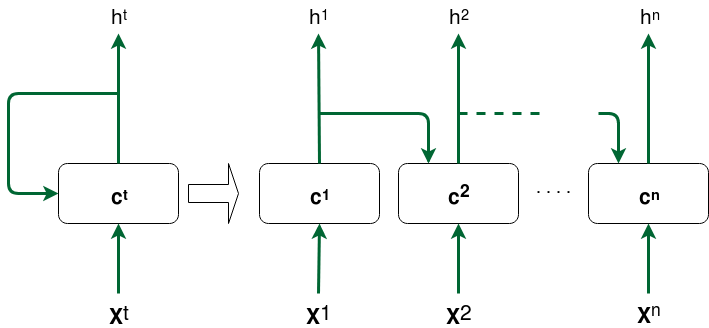
\includegraphics[width=\textwidth]{report/figures/techniques/RNN.png}
            \caption{A recurrent neural network, shown in its compact form to the left, and in its unrolled form to the right.}
            \label{fig:RNN}
        \end{figure}
    
        One of the downfalls of the RNN is that as the depth of the network grows with the number of time steps. This introduces two problems known as vanishing and exploding gradient. This phenomenon is explained in detail in \cite{Pascanu}. The short version is that as the number of time steps grows, the size of the network grows. This means that the number of computations in the backpropagation algorithm also grows. It can be shown that each of the n layers as seen in Figure \ref{fig:RNN} gets its parameters updated as a partial derivative of the cost function for its prediction, in addition to the partial derivative of the next network. The exploding or vanishing gradient problem can be found by examining how $\frac{\partial \bm x_t}{\partial \bm x_k}$ is calculated. The following derivation from \cite{Pascanu},
        \begin{align}
            \frac{\partial \mathcal{E}}{\partial \theta} = \sum_{1\leq k \leq t}\frac{\partial \mathcal{E}_t}{\partial \theta} \nonumber \\
            \frac{\partial \mathcal{E}_t} = \sum_{1\leq k \leq t}\frac{\partial \mathcal{E}_t}{\partial \bm{x_t}} \frac{\partial \bm{x_t}}{\partial \bm{x_k}}\frac{\partial \bm{x_k}}{\partial \theta} \nonumber \\
            \frac{\partial \bm{x_t}}{\partial \bm{x_k}} = \prod_{t \geq i\geq k} \frac{\partial \bm{x_i}}{\partial \bm{x_{i-1}}}\label{eq:rnn_xprod}, 
        \end{align}
        shows how the partial is calculated. As seen in Equation \ref{eq:rnn_xprod} the partial of $\bm x_t$ becomes a product of all internal states of the timesteps between t and k. Hence, if these values are $\geq1$ the gradient will grow, and if they are $\leq 1$ they will decrease. As the number of timesteps grows, the gradient then runs the risk of either explode or vanish. A possible solution to this problem is presented in the next section.  
    
    \subsection{Long short term memory recurrent neural networks}
        Long Short-Term Memory RNN or LSTM RNN is an extension of the RNN seen in subsection \ref{subsubsec:RNN}. The idea behind it is to create loops where the gradient can flow for long durations, and hence solving the issue with vanishing and exploding gradients. LSTM was introduced in \cite{Hochreiter1997}, and has been found very successful in many different applications. Figure  \ref{fig:lstm} shows the building blocks of the LSTM. The LSTM consist of four internal layers, forget layer, input gate layer, two tanh layers and the output layer. All of those layers are a separate NN layer. The previous cell state is fed in at the top of the LSTM. The previous state is kept based on the previous output $\bm h^{t-1}$ and the current input $\bm x^t$ which is fed through the forget layer. If none of the previous states is seen as relevant, the output will be a vector of zeros. If the previous state is seen as extremely important, it will output a vector of ones. Next, the information in the new input is analyzed. The tanh layer creates an estimation of the current LSTM state $\bm c^t$ based on $\bm h^{t-1}$ and $\bm x^t$. This value is then scaled by the output of a sigmoid layer $\bm I^t$ which decides which of the internal states to update. $\bm c^t$ is then computed as a function of the previous state and the new state estimation. The output is calculated by sending the current cell state through a tanh layer before a sigmoid layer decides which part of the cell state to output.  
        
        \begin{figure}
            \begin{minipage}[b]{0.99\linewidth}
            \centering
            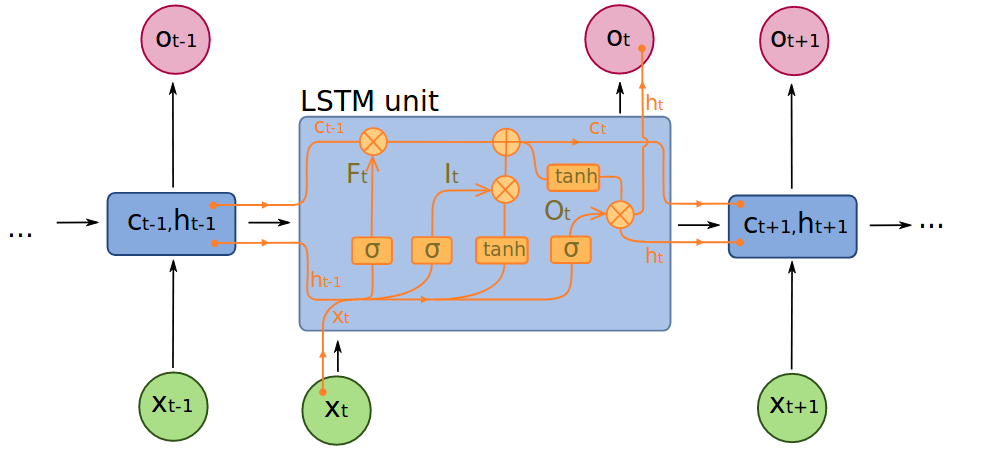
\includegraphics[width = \textwidth]{report/figures/techniques/lstm.png}
            \caption{A lstm network, By François Deloche \footnote{Lisenced under CC BY-SA 4.0, \url{https://commons.wikimedia.org/wiki/File:Long_Short-Term_Memory.svg}}} 
            \label{fig:lstm}
            \end{minipage}
        \end{figure}
        
        
        LSTM is proposed as a scheme for anomaly detection in \cite{Malhotra2016} and \cite{Malhotra}. It is shown that the scheme is working for both periodic and aperiodic time series. LSTM RNN has been successfully used for handwritten text recognition and speech recognition. The paper proposes an encoder-decoder scheme designed for anomaly detection. A time series is encoded and then decoded back to reconstruct the input series. The reconstruction error, the error between the input and the reconstructed input is then used to identify outliers. In the training phase, the system is only shown normal data. Hence it only learns to reconstruct the normal system behavior. The network should then not be able to reconstruct anomalous data as good as with normal data. The paper concludes that LSTM networks can be a viable approach for anomaly detection. It also shows promise in detecting anomalies from unpredictable time-series.      
        